\section{Backhual Algorithm and Evaluation}
\label{sec:whitemesh}

% Organization of the Sec
In this section, we study the channel assignment problem jointly use  WiFi and white space 
bands in concert of backhual tier. We then present our linear programming model and 
heuristic-based measurement-driven algorithm to address the problem. 
 
\subsection{Linear Programming Formulation}
\label{subsec:linearopt}


% Metrics
A wireless network is designed to satisfy the traffic demand from the users. Wireless networks are 
operated and maintained by vendors, such as AT\&T, T-Mobile, who charge the customers based on their 
data through Internet. In practice, the traffic demand of the user obey Poisson process~\cite{saaty1961elements}, 
The traffic demand of the users delivered to or from Internet are noted as served traffic flow. 
In particular the served traffic flow $X$, is represented in Eq.~\ref{eq:goodput}:
\begin{equation}
\label{eq:goodput}
X=\sum_{w \in W, v \in V}T(w,v)
\end{equation}
$T(w,v)$ nodes all delivered traffic between access point $v \in V$ and gateway node $w \in W$.


%To clarify the problem and approach the optimization solution of the problem, 
Here, we present a linear programming formulation to approach the optimal channel assignment in WhiteMesh. 
We leverage the nodes into the set of available access points ($V$), gateways ($W$) who convert the traffic to the 
Internet. The available bands ($B$) are pre-known as input. The conflict graph $I$ is given 
as parameters. The achieved channel capacity $\delta_b$ is from the  activity level measurements processing in~\ref{eq:intercap}. 


\noindent
{\bf Sets:}
\begin{tabular}{ll}
$V$ & set of nodes \\
$B$ & set of bands \\
\end{tabular}

\noindent
{\bf Parameters:}\\
\\
%\vspace{0.1in}
%\begin{tabular}{lll}
\begin{tabular}{llp{3.4cm}}
%\hline
$\delta^b$ & $b \in B$ & Achieved capacity of band $b$ in target area\\
%\begin{tabular}{llp{2.8cm}}
$I_{ij,lm}^b$ & $(i,j,l,m) \in V, b\in B $ & Protocol Interference of link $(i,j)$ on band $b$ brought by link $(l,m)$\\
%\hline
%\end{tabular}\\
%\begin{tabular}{llp{2.8cm}}
$W_i$ & $i \in V\ binary$ & Gateway marked with access point set\\
%\hline
%\end{tabular}\\
%\begin{tabular}{llp{2.8cm}}
$D_{d}$ & $i \in V\ $ & Downlink demand of node i\\
%\hline
%\end{tabular}\\
%\begin{tabular}{llp{2.8cm}}
$D_{u}$ & $i \in V\ $ & Uplink demand of node i\\
%\hline
\end{tabular}

The variable time share represents the assigned percentage of a single link transmitting time as~$\alpha_{i,j}^b$ 
for link $i,j$ between node $i$ and node $j$ in band $b$. The two variables, $uy_{i,j,k}^{b}$ and $dy_{i,j,k}^{b}$ 
are defined as uplink and downlink flows:

\noindent
%\vspace{2pt}
{\bf Variables:}\\
\\
%\vspace{1pt}
\begin{tabular}{llp{3cm}}
$0\le \alpha_{ij}^b \le 1$  & $b\in B, (i,j) \in N$ & 
Time share of link $(i,j)$ on band $b$\\ 
$0\le uy_{i,j,k}^b$ & $(i,j,k) \in V, b \in B$ & 
Uplink flow of node $k$ on link $(i,j)$ at band $b$ \\ 
$0\le dy_{i,j,k}^b$ & $(i,j,k) \in N, b \in B$ & 
Downlink flow of node $k$ on link $(i,j)$ at band $b$ \\ 
\end{tabular}
\vspace{1pt}

% FIXME talk about NT calculation
The objective is to maximize the served traffic flow ($X$) defined in Eq.~\ref{eq:goodput}.

\noindent
{\bf Objective:}
\begin{align}
& Max \sum_i\sum_j\sum_k\sum_b(uy_{i,j,k}^b+dy_{j,i,k}^b) \;\ When \; w_j=1 
%& Max \sum_i\sum_j\sum_b(\frac{1}{\sum_{l,m}\alpha_{i,j}^b\times I_{ij,lm}})
\end{align}

In the LP, the constraints are presented as connectivity, uplink, and downlink sections here:  

\noindent
%{\bf Constraints:}
{\bf Connectivity Constraints:}
\begin{align}
\label{opt:1}
& \alpha_{i,j}^b + \alpha_{j,i}^b + \sum_l\sum_m(\alpha_{l,m}^b \cdot I_{ij,lm}^b) \leq \delta^b, i\neq j \\
\label{opt:2}
& \sum_i uy_{i,j,k}^b + \sum_i dy_{i,j,k}^b \leq \delta^b \cdot \alpha_{j,k}^b 
\end{align}
\noindent
{\bf Uplink Constraints:} 
\begin{align}
\label{opt:3}
& \sum_k \sum_b uy_{i,k,i}^b \leq D_{ui}  \; ; w_k=0, i \neq k \\
\label{opt:4}
& uy_{i,j,k}^b \cdot w_k = 0 \\
%\label{opt:5}
%& \sum_i\sum_b uy_{i,j,k}^b - \sum_m\sum_b uy_{j,m,k}^b = 0 \; when \; w_k=0, i\neq k\\
\label{opt:6}
& \sum_{i\neq j}\sum_b uy_{i,j,k}^b = \sum_{m\neq j} \sum_b uy_{j,m,k}^b \; ;w_j = 0\\
\label{opt:7}
& uy_{i,j,i}^b=0 
\end{align}
\noindent
{\bf Downlink Constraints:} 
\begin{align}
{\bf}
\label{opt:8}
& \sum_k \sum_b dy_{i,k,i}^b \leq D_{di} \; \; ; w_k=0 \\
\label{opt:9}
& dy_{i,j,k}^b =0  \; ;w_k=1 \\
%\label{opt:10}
%& \sum_j\sum_b dy_{i,j,k}^b - \sum_m\sum_b dy_{i,k,m}^b \geq , i \neq k \\
\label{opt:11}
& \sum_{i\neq j} \sum_b dy_{i,j,k}^b = \sum_{m \neq j} \sum_b dy_{j,m,k}^b   \; ; w_j=0, i \neq k \\
\label{opt:12}
& dy_{i,i,j}^b=0
\end{align}

In these constraints, (\ref{opt:1}) represents the total time assigned for the incoming, outgoing flows 
and the interfering time should all be less than 1. Constraint (\ref{opt:2}) represents the incoming and 
outgoing wireless traffic flow are less than the capacity assigned for link $i,j$. Uplink constraints 
(\ref{opt:3}) and (\ref{opt:4}) represent that the total traffic flow on link $i,j$ from $i$ is less than 
the demand of node $i$. Constraints (\ref{opt:6}) and (\ref{opt:7}) restricts the sum of incoming data 
flows for a given access point $k$ equal to the total outgoing flows from the node. Downlink constraints 
(\ref{opt:8}) and (\ref{opt:9}) represent similar restrictions as (\ref{opt:3}) and (\ref{opt:4}), but 
in the downlink direction.  Constraints (\ref{opt:11}) and (\ref{opt:12}) are downlink versions of 
(\ref{opt:6}) and (\ref{opt:7}).
Since linear programs model for multiple channels has been proved to be NP-hard~\cite{yuan2006cross}. 
In this work, we choose small size of cases to achieve the optimal solution and validate other
approaches in.






% PEN part 
%\subsection{Path Interference Induced on the Network}
\label{subsec:PEN}

In WhiteMesh networks, multihop paths can be intermixed with WiFi 
for more spacial reuse and white space bands with less hops.  
To deal with the trade-off, we consider
analyze the band choices reduce the number of hops along a path and the 
aggregate level of interference that hop-by-hop path choices have
on the network (i.e., Path Interference induced on the Network).

Mesh nodes closer to the gateway generally achieve
greater levels of throughput at sufficiently high offered loads. 
To combat such starvation effects, we treat each flow with equal priority in the network when
assigning channels. In the worst case, all nodes along a particular path have equal 
time shares for contending links (i.e., intra-path interference).
We start the channel assignment assuming that $h$ mesh nodes are demanding
traffic from each hop of an $h$-hop path to the gateway. If each link along the 
path uses orthogonal channels, then each link could be active simultaneously,
otherwise they will complete with each other. 
We note each node along the path had traffic demand $T_d$, obviously the bottleneck 
link along the path would be the one closest to the gateway, and then next. 
Thus, the total traffic along the path $h \cdot T_d$ must be less than the 
bottleneck link's capacity $\delta$ estimated from the measurements. In such a scenario, the $h$-hop mesh node 
would achieve the minimum served demand, which we define as the network efficiency. 
In general, the active time per link for an $h$-hop mesh node can be represented 
by $1,\frac{h-1}{h},\frac{h-2}{h}\cdots \frac{1}{h}$. The summation of all active 
times for each mesh node along the path is considered the intra-path network cost.

Considering only intra-path interference, using lower carrier frequencies allows a
reduction in hop count and increase in the network efficiency of each mesh node along
the $h$-hop path. However, a lower carrier frequency will induce greater interference
to other paths to the gateway (i.e., inter-path interference). 
Fig.~\ref{fig:interferencerange} depicts such an example where
links in different bands are represented by circles for 450 MHz, rectangles for
2.4 GHz, and triangles for the nodes which can choose between the two.
Nodes $A$ and $C$ could be connected through two 2.4-GHz links or a single 450-MHz link.
With 2.4 GHz, the interfering distance will be less than using 450 MHz. For example, only 
link $D,E$ will suffer from interference, whereas $H,I$ would not. However, with 450 MHz,
link $A,C$ would interfere with links $F,G$, $M,L$, and $K,J$. At each time unit, the number of
links interfering with the active links along a path would be the inter-path network cost.

When an $h$-hop flow is transmitted to a destination node, it prevents 
activity on a number of links in the same frequency via the protocol model. 
The active time on a single link can be noted as 
$\frac{T}{\gamma_h}$. 
An interfering link from the conflict matrix $F$ counts as $I_h$ per unit time
and contributes to the network cost in terms of:
$\frac{hT}{\gamma_1}\cdot I_1 + \frac{(h-1)T}{\gamma_2}\cdot I_2 \cdots \frac{T}{\gamma_h}\cdot I_h$.
Then, the traffic transmitted in a unit of network cost for the $h$-hop node is:
\begin{equation}
\label{eq:originpen}
E_{\eta}=\frac{T}{\sum_{i \in h}\frac{(h-i+1)\cdot T}{\gamma_i}\cdot I_i }
\end{equation}
Using network efficiency, the equation simplifies to:
\begin{equation}
\label{eq:pen}
E_{\eta}=\frac{\gamma}{\sum_{i \in h} (h-i+1)\cdot I_i}
\end{equation}

The network efficiency is the amount of traffic that could be 
offered on a path per unit time. With multiple channels from the same band,
$I_i$ will not change due to the common communication range. With multiple
bands, $I_i$ depends on the band choice due to the communication range diversity.  
This network efficiency jointly considers hop count and interference. We define
the Path Interference induced on the Network (PIN) as the denominator of Eq.~\ref{eq:pen},
which represents the sum of all interfering links in the network by a given path. 
PIN is used to quantify the current state of channel for channel assignment
across WiFi and white space bands.
To determine when the lower carrier frequency will be better than two or more hops at a
higher carrier frequency, we consider the average interference $\bar{I}$ of a given path
at the higher frequency.  The problem could be formulated as:
\begin{equation}
\label{eq:benefit}
\frac{\gamma}{\frac{h(h-1)}{2}\cdot \bar{I}+I_x} \geq \frac{\gamma}{\frac{h(h+1)}{2}\cdot \bar{I}}
\end{equation}

Here, from Eq.~ref{eq:benefit} when $I_x \leq 2\cdot h\bar{I}$, the performance of a lower-frequency link  
is better than two higher-frequency hops for the same destination node. $I_x$ is also a parameter of hop count 
in Eq.~\ref{eq:pen}. When the hop count is lower which closer to the gateway node, the threshold 
would be more strict since the interference would have a greater effect on the performance.



\subsection{Path Interference Induced on the Network}
\label{subsec:PEN}

In WhiteMesh networks, it is possible that multihop paths intermixed with WiFi for more spatial reuse 
and white space bands with less hops. We analyze the band choices reducing the number of hops along 
a path and the aggregate level of interference that hop-by-hop path choices have on the network (i.e., Path 
Interference induced on the Network).

Mesh nodes closer to the gateway generally achieve greater levels of throughput at sufficiently high 
offered loads. To combat such starvation effects, we treat each flow with equal priority in the network 
when assigning channels. In the worst case, all nodes along a particular path have equal time shares for 
contending links (i.e., intra-path interference). We start the channel assignment assuming that $h$ mesh 
nodes are demanding traffic from each hop of an $h$-hop path to the gateway. If each link along the path 
uses orthogonal channels, then each link could be active simultaneously, otherwise they will complete with 
each other. We note each node along the path had traffic demand $T_d$, obviously the bottleneck link 
along the path would be the one closest to the gateway, and then next. Thus, the total traffic along the 
path $h \cdot T_d$ must be less than the bottleneck link's achieved capacity $\delta$ estimated according 
to the measurements. The $h$-hop access point would achieve the minimum served demand, which we define as the 
network efficiency. In general, the active time per link for an $h$-hop access point can be represented by 
$1,\frac{h-1}{h},\frac{h-2}{h}\cdots \frac{1}{h}$. The summation of all active times for each access point 
along the path is considered the intra-path network cost.


Using lower carrier frequencies allows a reduction in hop count and increase the network efficiency of each 
access point along the $h$-hop path by reducing the interference among the links of the path. However, a lower 
carrier frequency will induce greater interference to other paths to the gateway (i.e., inter-path interference). 
When an $h$-hop flow is transmitted to a destination node, it prevents activity on a number of links in the 
same frequency via the protocol model. The active time on a single link is noted as $\frac{T}{\gamma_h}$. 
An interfering link from the conflict matrix $F$ counts as $I_h$ per unit time and contributes to the network 
time cost in terms of:
$\frac{hT}{\gamma_1}\cdot I_1 + \frac{(h-1)T}{\gamma_2}\cdot I_2 \cdots \frac{T}{\gamma_h}\cdot I_h$.
Then, the traffic transmitted in a unit time of network cost for the $h$-hop node is:
\begin{equation}
\label{eq:originpen}
E_{\eta}=\frac{T}{\sum_{i \in h}\frac{(h-i+1)\cdot T}{\gamma_i}\cdot I_i }
\end{equation}
Through network efficiency, the equation simplifies to:
\begin{equation}
\label{eq:pen}
E_{\eta}=\frac{\gamma}{\sum_{i \in h} (h-i+1)\cdot I_i}
\end{equation}

Network efficiency is the amount of traffic that could be offered on a path per unit time. With 
multiple channels from the same band, $I_i$ will not change due to the common communication 
range. With multiple bands, $I_i$ depends on the band choice due to the communication range 
diversity. Network efficiency jointly considers hop count and interference in the paths. We define
the Path Interference induced on the Network (PIN) as the denominator of Eq.~\ref{eq:pen}.
The parameter represents the sum of all interfering links in the network by a given path. 

PIN is used to quantify the current state of channel for channel assignment across WiFi and 
white space bands. To determine when the lower carrier frequency will be better than two or 
more hops at a higher carrier frequency, we consider the average interference $\bar{I}$ of 
a given path at the higher frequency. The problem could be formulated as:
\begin{equation}
\label{eq:benefit}
\frac{\gamma}{\frac{h(h-1)}{2}\cdot \bar{I}+I_x} \geq \frac{\gamma}{\frac{h(h+1)}{2}\cdot \bar{I}}
\end{equation}

Here, from Eq.~\ref{eq:benefit}, when $I_x \leq 2\cdot h\bar{I}$, the performance of a 
lower-frequency link has better network efficiency than two higher-frequency hops for 
the same destination node. $I_x$ is also a parameter of hop count in Eq.~\ref{eq:pen}. 
When the hop count is lower which closer to the gateway node, the threshold would be 
more strict since the interference would have a greater effect on the performance.


\subsection{Band-based Path Selection (BPS) Algorithm}
\label{subsec:BPS}

\begin{figure}
\vspace{-0.0in}
\centering
\includegraphics[width=74mm]{figures/interferencerange2}
\vspace{-0.1in}
\caption{Example WhiteMesh topology with different mesh-node shapes 
representing different frequency band choices per link.}
\label{fig:interferencerange}
\vspace{-0.1in}
\end{figure}

% Intra network interference
In Fig.~\ref{fig:interferencerange}, the access point $A$ could connect to access point $C$ 
relayed by node $B$ at 2.4 GHz, or directly connect to $C$ at 450 MHz. If 2.4 GHz were 
chosen, link $D,E$ is able to reuse 2.4 GHz when they are out of the interference range. 
However, in backhual tier network if link $A,C$ used 450 MHz, a lower hop count would 
result for the path, but lower levels of spatial reuse also result (e.g., for link $D,E$). 
While the issues of propagation, interference, and spatial reuse are simple to understand, 
the joint use of white space and WiFi bands to form optimal WhiteMesh topologies is 
challenging since the optimization is based on the knowledge of prior channel assignment 
which is not available before the work has been done.

In the backhaul tier, we formulate the problem with a graph model. A connectivity graph $C$ is 
formed for each band in $B$ such that $C=(V,L,B)$. If the received signal for a given band is 
above an interference-range threshold, then contention occurs between nodes. We extend the conflict 
matrix in~\cite{tang2005interference} related to various interference per band according to 
$F=(E_{i,j},I_{Set},B)$, where $E_{i,j}$ represents the link and $I_{Set}$ includes all the links 
are physically inside the interference range $D_r$ when operating on each band $b \in B$.

Therefore, the problem we model is: to choose the connectivity graph $C'$ which maximizes the served 
traffic flow from the access tier. A key challenge is that selecting the optimal channels from the 
set $B$ leads to a conflict graph $F$ which cannot be known {\it a priory}. 

%Previous works have proposed 
%several coloring, cluster-independent set, mixed linear integer methodology for a single band $b$ 
%~\cite{peng2012efficient,tang2005interference,doraghinejad2014channel}. 
%However, these works fails to address a reduction in hop count or an increase in spatial reuse and 
%channel occupancy for a set of diverse bands $B$.

\begin{algorithm}[t]
    \small
\caption{Band-based Path Selection (BPS)}
\begin{algorithmic}[1]
\label{algorithms:bps}
\REQUIRE  ~~\\
	$M$: Set of access points\\
	$G$: Set of gateway nodes\\
	$C$: Communication graph of potential links among all nodes\\
	$I$: Interference matrix of all potential links \\
	$B$: Available frequency bands \\
	$\delta$: Measurements based Channel Capacity
\ENSURE ~~\\    
$CA$: Channel Assignment of the Network\\
\STATE Rank access points in Set $M$ according to physical distance from gateway nodes $G$
\STATE Initialize $S_{curr}=G$, $N_{srv}=\emptyset$, $N_{unsrv}=M$,$I_{active}=\emptyset$
\WHILE {$N_{srv}=!M$}
\STATE Select node with largest distance to gateway
\STATE Find the adjacency matrix across band combinations $A_c$
\FORALL{$A_{i}\in A_c$}
\STATE Find the shortest path $SP_i$ in mixed adjacency matrix A 
\FORALL{Link $l \in SP_i$, ordered from gateway to access point}
\STATE Find the least interfering path with measured $\delta \times E_n$
\STATE If equally-interfering links, choose higher frequency
\STATE Calculate the path interference of $SP_i$
\ENDFOR
\STATE Store the shortest path $SP_i$ as $SP$
\ENDFOR
\STATE Assign the path in the network\\
		\STATE Update $N_{srv},N_{unsrv}$
		\STATE Update $I_{active}$ from $I$
\ENDWHILE \\
Update $CA$ as the locally-optimal solution\\
\end{algorithmic}
\end{algorithm}



We design a Band-based Path Selection (BPS) algorithm shown in Alg.~\ref{algorithms:bps}. 
The algorithm first chooses the access point that has the largest physical distance from the 
gateway nodes in the network to reduce the total time cost of the network by improving the 
worst one. When a path is constructed for the access point with the greatest distance, all 
subsequent access point along the path are also connected to the gateway. 
In large-scale mesh networks, the complexity makes it impractical to traverse all the 
paths with different combination of bands from an access point to any gateway node. It has been 
proved as a NP-hard problem. However, based on the discussion in subsection~\ref{subsec:PEN}, 
if two paths have the same number of used bands along those paths, then the path with the 
least hops is likely to have the greatest performance and is chosen. Similarly, if two path 
have the same path interference, we choose the path which has higher-frequency links to keep 
the potential improvement of spatial reuse. Thus, the next step of the algorithm is to find 
the shortest path across band combinations.

In the algorithm, compared to the number of access points, the amount of channels $N_B$ in
different bands is small. The time complexity of calculating the combination is $O(2^{N_B})$. 
Finding the shortest path in Dijkstra algorithm will cost $O(N_E^2)$~\cite{golden1976shortest}, 
where $N_E$ is the set of possible links in the network, and as a result, the total complexity 
would be $O(N_E^2\cdot 2^{N_B})$. 
The algorithm will compare the PIN of the candidate paths and select the path with the 
least interference channel induced on the network for the source access point.
The algorithm updates the channel assignment of the network after the path is chosen.
Then, the served nodes, activated links, and radio information are refreshed. 
The process will repeat iteratively to assign channels for all the access points in the
network.

The complexity of assigning a channel for an access point is $O(N_E^2\cdot2^{N_B})$ 
if all the nodes are connected to gateway nodes ($N_E={n \choose 2}$ which is $O(N_V^2)$). 
The complexity of assigning an access point is $O(N_V^4\cdot2^{N_B})$.
To assign {\it all} the access points in the network, the complexity would be 
$O(N_V^5\cdot2^{N_B})$. The complexity is polynomial time of the number of traffic 
demands points (mesh group) for a wireless network assignment.


\subsection{Experimental Evaluation Setup}
\label{subsec:design}
% Simulation Setup
The WhiteMesh networks has the diversity in propagation from the lowest white space channels 
(tens to hundreds of MHz) to the highest WiFi channels (multiple GHz). We consider a wide range 
of propagation characteristics from four different frequency bands to set up the experimental 
evaluation. We take 450 MHz and 800 MHz of white space bands and 2.4 GHz and 5.2 GHz of WiFi bands
data from measurement work in Section~\ref{sec:measurements}.

% Network Setup
The measurements map the experimental setup according to the population distribution across 
different cities. We input the measurements to both the LP and heuristic-based algorithm to compare 
the performance in various scenarios. The communication threshold is set as -100 dBm. The 
communication range is normalized with the highest frequency of 5.2 GHz. Then the communication 
range of 450 MHz, 800 MHz, 2.4 GHz, and 5.2 GHz would be normalized as 12.8, 6.2, 2.4, and 1, 
respectively in Friis model as Eq.~\ref{eq:friis}. 
The interference range is set as twice that of the communication range~\cite{raniwala2005architecture}. 
We deploy static wireless mesh networks of $n$ access points along a regular grid with a normalized 
distance of 0.8 between rectangular edges. The gateways are chosen through a typical cell hexagon 
deployment method based on 2.4 GHz~\cite{meguerdichian2001exposure}. Unless otherwise, specified 
in the analysis, all four bands are used in the WhiteMesh topology studied. For practical application 
scenarios, more channels could be involved in the algorithms.


% Traffic generation
The traffic demand aggregated by an access point is independent to others and obey Poison distribution
during unit time. 
In the simulation, we generate an equal number of access points (including both gateway nodes and 
access points) Poison random numbers with an mean $\lambda$ according to the population distribution 
for the target area. Then we map the number to the traffic demand for each access points in the 
target area.
% Served traffic flow calculation
As mentioned previously, the achieved channel capacity of gateway nodes has been shown to be the bottleneck in mesh 
networks~\cite{robinson2010deploying}. Moreover, served traffic flow is affected by access point placement, 
gateway placement, routing, and channel assignment, etc. For the purposes of our analysis, we specifically 
calculate the served traffic flow through the greedy strategy. 
The channel assignment process make the network under a tree based structure. We start to serve the traffic 
demand from the gateway nodes. Mesh nodes that have less hop count path to the gateways are served first. 
When access points have the same number of hop count, the least interfering access points are chosen to 
reduce the cost for the whole network. The process repeats until no remaining traffic demand of users 
or no remaining channel capacity on any path.

The impacts of network size, bands availability, and channel occupancy on WhiteMesh networks are 
investigated in the simulation. The achieved channel capacity of the target area is calculated from the 
measurements according to the population distribution of the cities. Assuming 10\% of the residents will use the 
service. An individual user would have a 100 KB/s traffic demand on average. 
We assign the traffic demand to users under the same Poison setting and run the analysis 
of each case 20 times. To approach the served traffic flow up-bound, we relax our LP model to only keep 
the link capacity constraints, given the traffic demand of the access points as a parameter to achieve 
the maximum throughput at the gateways. We further compare BPS with the 
{\it (i)} Common Channel Assignment (CCA) from~\cite{draves2004routing},
{\it (ii)} Breath First Search Channel Assignment (BFS-CA) from~\cite{tang2005interference}
under the same setup.
CCA~\cite{draves2004routing} algorithm assigns a common channel for two nodes when both of them 
share free radios working in the same channel. In BFS-CA~\cite{tang2005interference} algorithm, 
a node will search all the available single-hop connections then choose the one has the largest 
free capacity for a new assignment. 
These two methods are designed for multi-channel scenarios assuming the existing 
links are equal when there is no assignment on the channel. 



\subsection{Experimental Analysis of WhiteMesh Backhaul}
\label{subsec:wmanalysis}

\subsubsection{Network Size \& Bands Effect}

% ILP bound
Typically, the traffic patterns of access points from users are diverse with
the download direction dominating the total traffic demand (e.g., consider
service agreements for cellular data or Internet connectivity). 
Hence, to simplify the analysis and scale the LP Bound to larger network 
sizes, we only consider the download traffic while maintaining the simulations.

We investigate the network sizes impacts on wireless WhiteMesh network. 
The number of access points is varied from $16$ to $64$ in the aforementioned 
regular grid. As the network size grows, so too does the number of gateways
through the hexagon gateway nodes deployment. Fig.~\ref{fig:varysize} shows 
the served traffic flow when the population distribution is 500 $ppl/km^2$ 
for the LP formulation and the heuristic-based algorithms: 
{\it (i)} Common Channel Assignment (CCA) from~\cite{draves2004routing},
{\it (ii)} Breadth First Search Channel Assignment (BFS-CA) from~\cite{ramachandran2006interference},
{\it (iii)} our algorithm BPS (Section~\ref{subsec:BPS}).


\begin{figure}[t]
\centering
\subfigure[Average Population Distribution = 500 $ppl/km^2$]{
\label{fig:varysize}
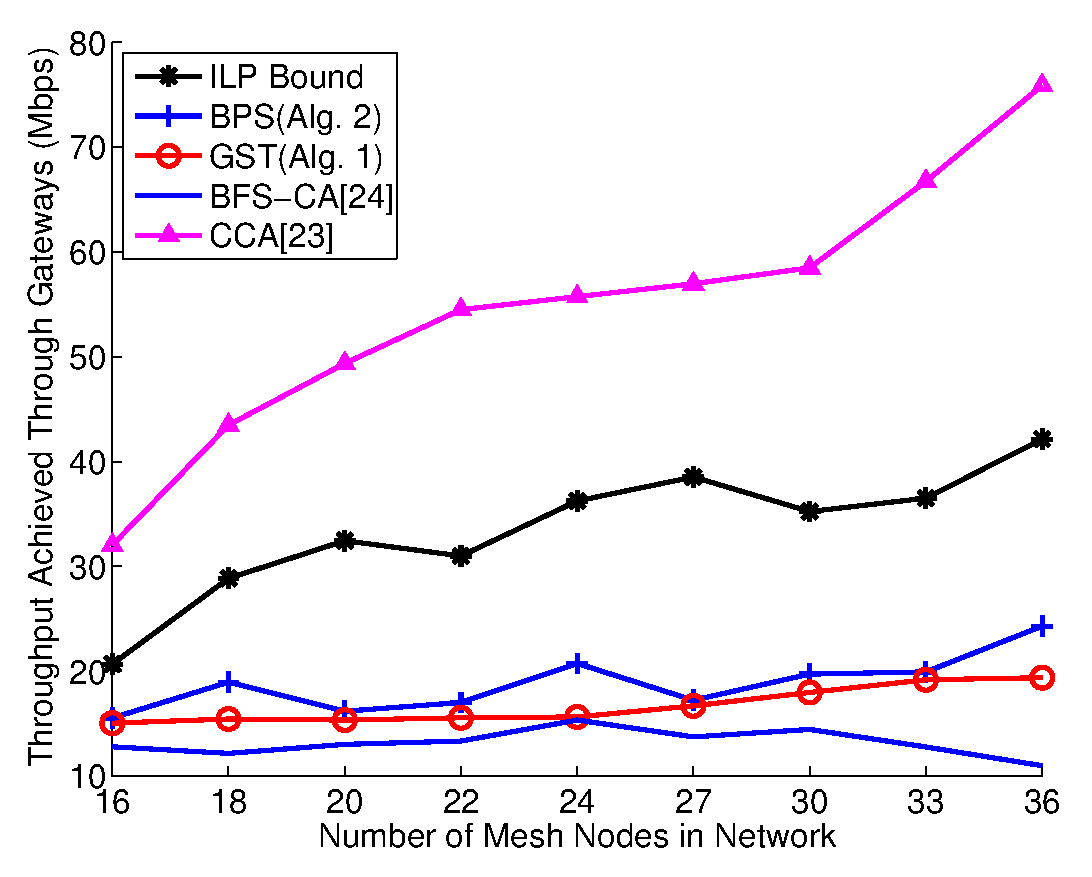
\includegraphics[width=1.6in]{figures/varysize}}
\subfigure[Varying Load, 49-Nodes Regular Grid]{
\label{fig:maxtpt}
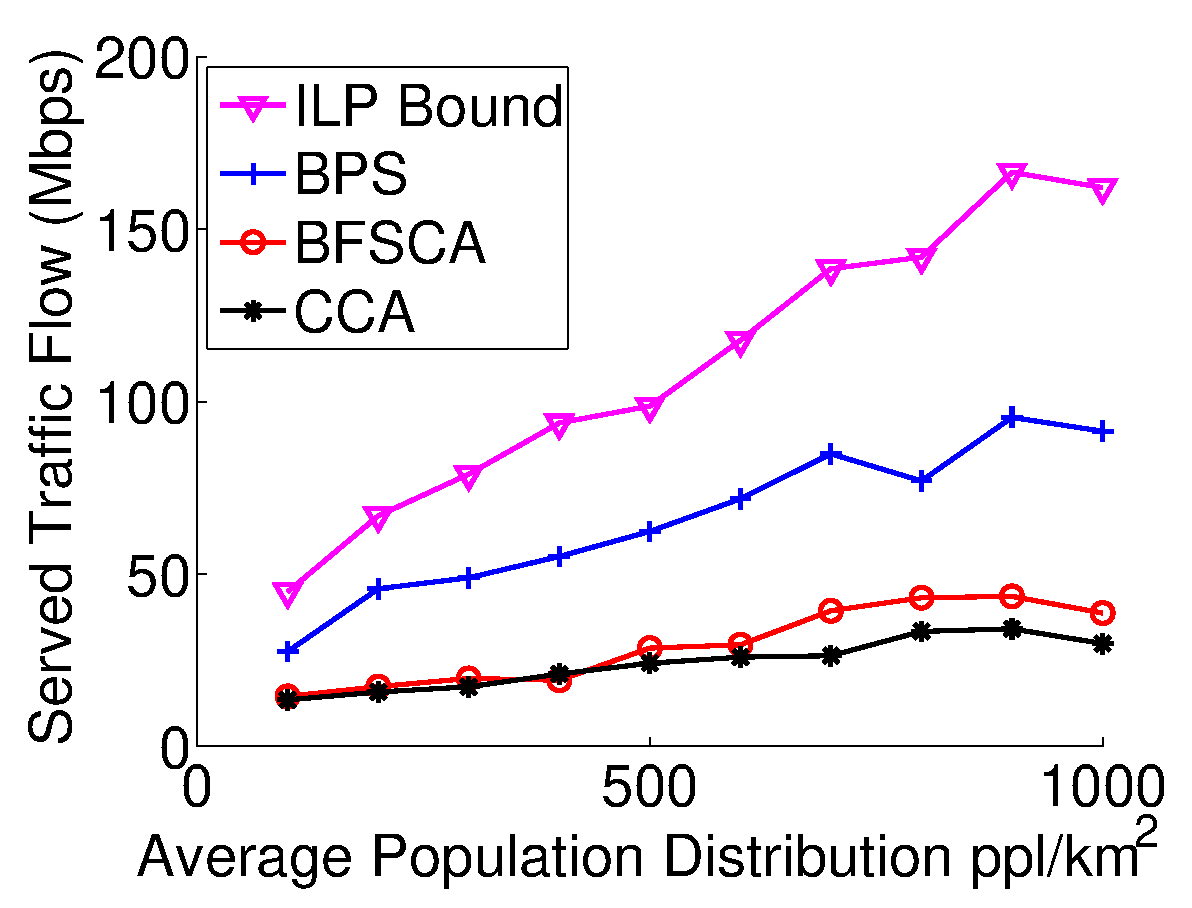
\includegraphics[width=1.6in]{figures/maxtpt.eps}}
\hfill
\caption{Performance in terms of served traffic flow for various offered loads, network sizes, and configurations of WiFi or white space (WS) channels.}
\label{fig:all3figs}
\vspace{-0.3in}
\end{figure}
%\end{figure*}

In Fig.~\ref{fig:varysize}, we observe as the network size increase, the performance
gap among BPS and CCA/BFS-CA increase. The network size represents the target area size. 
The multiband wireless network has similar communication and interference performance with 
the multi-channel wireless network since all the nodes are located in a limited space where 
could be communicated/interfered by all the bands. 
As network size increase, the connection/interference variation among multiple bands makes 
the performance of multi-channel algorithms stay in low level. The LP Bound shows what 
could be expected, that an increasing number of gateways/access points produce an increase in 
total served traffic flow. However, we observe that CCA, BFS-CA algorithms are not able 
to achieve such behavior for various reasons. CCA fails to employ the communication range 
variation and find the most efficient hop connections which increase the average hop count. 
BFS-CA optimizes the first connection hop from the gateway, but fails to deal the whole path 
from the gateway to destination node. Conversely, BPS alleviates the strain on these first-hop, 
bottleneck links, achieving average 76\% of the LP Bound. The gap of BPS to the LP is part from 
that the BPS only considers static one path to a gateway node for each access point, whereas the 
LP allows multiple paths to the gateways. For BPS and other heuristic-based algorithms the dynamic 
assignment could be implemented through updating the assignment in a short term.

\begin{table*}
\centering % centering table 
\begin{tabular}{|c|c|c|c|c|c|c|c|c|c|c|c|} % creating 12 columns 
\hline %\hline % inserting double-line 
%Bands     & \multicolumn{3}{c|}{Dallas} & \multicolumn{3}{c|}{Weatherford} & \multicolumn{3}{c|}{Millsap} \\% [0.5ex]
%\hline % inserts single-line 
% Entering 1st row 
 \multirow{2}{*}{Frequency Bands} & \multicolumn{9}{|c|}{Population Distribution $ppl/km^2$} \\
\cline{2-10}
		& 1500 & 1000 & 500 & 300 &  200 & 150 & 100 & 20 & 10 \\ % [0.5ex]
\hline % inserts single-line 
450 MHz &24.37	&25.83  &23.77	&6.05 &12.50  &14.03 & 7.00 & 0.07 & 0.02 \\      
\hline % inserts single-line                                                                                                       
800 MHz &4.40 	&16.49  &4.77	&5.22&5.07 &4.43  & 3.87 & 4.20 & 3.60 \\      
\hline % inserts single-line                                                                                                      
2.4 GHz &15.87 	&34.95  &2.60	&2.03&2.03 &2.77  & 2.07 & 1.60 & 0.80 \\      
\hline % inserts single-line                                                                                                     
5.2 GHz &19.70	&35.46  &1.53	&1.93&1.93 &1.33  & 1.27 & 2.07 & 2.10 \\      
\hline % inserts single-line 
\end{tabular}    
\caption{Activity Level under Population Distribution} % title name of the table 
\label{tab:activitymeasurement}    
\vspace{-0.3in}
\end{table*}    

% additional Simulation set up
Then we investigate a different form of scalability in our analysis.  Namely,
we increase the average population distribution from 100 to 1,000 per $km^2$, while
maintaining a 49-node regular grid topology. The achieved channel capacity is mapped 
to the measurement results with the closest population distribution. 
%
%measurements has the same distance to the current set up, the lower population 
%measurement will be chosen, for instance, we map $400 ppl/km^2$ to $300 ppl/km^2$ 
%measurements as shown in Table.~\ref{tab:activitymeasurement}. 
%
Fig.~\ref{fig:maxtpt} shows that as the population distribution increases, the LP and 
BPS diverge greatly from the remaining algorithms. Similar to Fig.~\ref{fig:varysize}, 
the wireless channel capacity around a gateway is quickly saturated if the algorithm is 
not focused on preserving that resource. Another factor of the performance is the 
channel capacity, as population increase the achieved channel capacity vary in different 
bands. As the population reaches 1,000 $ppl$, the served traffic flow decrease due to the 
achieved channel capacity and the saturation of wireless channel capacity around the gateway
nodes. BPS has an average performance of 60\% of the LP Bound, on average. CCA and BFS-CA
fails to perform well with the jointly WiFi and white space wireless network. 

\begin{table*}
\centering % centering table 
\begin{tabular}{|l|c|c|c|c|c|c|c|c|c|c|c|} % creating 12 columns 
\hline %\hline % inserting double-line 
Bands/     & WiFi    & WS      & WS \& & WS \& &  WS \& & WS \& & WS \&      &  WS \&      & Multi-WS \& & Multi-WS \& & Multi-WS \& \\% [0.5ex]
Algorithms & Only    & Only    & WiFi  & WiFi  &  WiFi  & WiFi  & Multi-WiFi &  Multi-WiFi & WiFi        & WiFi        & Multi-WiFi  \\
\hline % inserts single-line 
% Entering 1st row 
WS (MHz)   &                                                        & 450,800 & 450 &  800  &  450   & 800               & 450    & 800      & 450,800     & 450,800     & 450,800     \\
\hline
WiFi (GHz) & 2.4, 5 &                                                             & 2.4 &  2.4  &  5   & 5               & 2.4, 5& 2.4, 5        & 2.4             & 5         & 2.4, 5     \\ % [0.5ex]
\hline
\hline % inserts single-line 
CCA~\cite{draves2004routing}                & 22.4   &  13.4  & 13.2    &12.5    & 16.9       & 23.2   &  24.1  &   30.6&  25.2  &       23.9       &   30.4          \\      
\hline % inserts single-line                                                                                                       
BFS-CA~\cite{ramachandran2006interference}  & 26.3   &  15.8  & 14.9    & 19.4   & 22.7       & 28.4   &  38.9  &   33.7&  30.1  &       27.4       &       36.6      \\      
%\hline % inserts single-line                                                                                                      
%GST (Alg. 1)                                                            & 11.6  &   6.6 & 9.3    &   15.1&   15.8        &  14.4  &   16.6   &    14.1  &   18.8            &  15.0           &    25.1         \\      
\hline % inserts single-line                                                                                                     
BPS (Alg. 1)                                & 41.2   & 34.1   &  38.2  & 40.0    & 35.4       & 42.8   & 58.4   &  64.9 &  54.4  &       51.9       &       63.1      \\      
\hline % inserts single-line 
\end{tabular}    
\caption{ Served Traffic Flow (Mbps) for various combinations of WiFi and Average Population Distribution = 500 $ppl/km^2$, Network Size = 49 access points).} % title name of the table 
% NEWClaim fix
\label{tab:2channelcombination}    
\vspace{-0.4in}
\end{table*}    


WhiteMesh networks may be deployed across a vast array of environments, from
rural to urban areas. Each of these areas will have varying amounts of user
demand traffic in proportion to the population densities. 
However, since a greater number of TV stations exist in urban areas, the available 
white space bands are often inversely related to the population density due to 
the FCC regulation~\cite{fccwhitespace}. To capture these varying degrees of demand 
and white space availability we consider three likely scenarios and one final 
scenario for comparison purposes: {\it (i)} two WiFi bands (2.4 and
5.2 GHz) channels with two white space channels (450 and 800 MHz), {\it (ii)} 
three channels in two WiFi bands (2.4 and 5.2 GHz) with one white space channel 
(450 MHz), {\it (iii)} Four channels in two WiFi bands (2.4 and 5.2 GHz) without 
any white space channels, and {\it (iv)} four channels in two white space bands 
(450 and 800 MHz) with no WiFi bands (for comparison).

Table~\ref{tab:2channelcombination} describes the served traffic flow 
for various scenarios of WiFi and white space bands with a offered load 
of 5 Mbps as Poison mean value from 500 $ppl/km^2$ in a regular 49-node grid. 
We study the performance of BPS in the four aforementioned scenarios of varying 
white space availability. In the simulation, we keep total 4 channels for each
method, such as in the combination of 2.4 GHz and 5 GHz, we put 2 channels in both 
bands. In the triple bands combinations, we set each band has a channel, and put the 
other channel in the highest frequency band. (In 2.4 GHz, 5GHz, 800 MHz combination, 
we put the extra channel other than the 3 channel each band in 5 GHz). 
% Justification
Immediately, we observe that the WiFi-only scenario has greater served traffic flow 
than the white-space-only scenario. This is due to the lack of spatial reuse achieved 
by white spaces bands. White space has larger communication range to shorten 
the hop counts as well as has larger interference reducing the spatial reuse. 
Another reason is that the achieved channel capacity of 500 $ppl/km^2$ in white 
space bands are worse than WiFi bands. These two reasons make the performance of 
white space only worse in all channel assignment methods applied here.
Interestingly, however, the joint use of both white space and WiFi bands has 
significant gains over the single type of band scenarios with the same number of 
channels (40\% greater than WiFi and 56\% over white space, on average). 

In 500 $ppl/km^2$ scenario, 5 GHz channel is cleaner than 450 MHz which makes 
the combination of 2 channels in 5 GHz, 1 channel in 2.4 GHz and 800 MHz has 
better performance than WiFi(2)+WS(2) in some cases. 


In Table ~\ref{tab:2channelcombination}, that with the same number of bands (2), 
the combination with similar propagation characters, the clean channels combination 
has better performance. With similar achieved channel capacity, lower frequency 
offers more option for connection path perform better in channel assignment. 
If we have one channel in a white space band and one channel in a WiFi band, then 
we could employ the advantages of both WiFi for spatial reuse and white spaces to 
reduce the hop count in channel assignment. 

\subsubsection{Access Tier Impacts on Backhaul Tier}

The density of access points increase proportional to the population 
density to offer enough access capacity for the users. Hence, the distance between the access points and the channel 
occupancy in backhaul tier channel assignment have to be counted. To investigate how the spacing variation 
and occupancy in the access tier impacts on the backhaul tier, we perform simulation on a 
49-node regular grid WhiteMesh network. 

In Fig.~\ref{fig:actspac}, we show the impacts of channel occupancy through 
the activity level and spacing variation on wireless white space mesh network. 
The spacing gap represents the access points density proportional to the 
population distribution. In the results, all the bands have the same activity 
level in the 49-nodes regular grid with normalized multiple spacing distance gap 
from 0.2 to 2.1 as discussed in Subsection~\ref{subsec:design}. In the 3-D figure, 
as the activity level increases, the served traffic flow decreases due to the reduction 
of achieved channel capacity. In the spatial dimension, when the nodes have extremely
small spacing, all the bands could not be leveraged spatial reuse, and the traffic 
arrived gateways is small. But as the spacing gap increases, the high frequency bands 
have greater spatial reuse bring higher served traffic flow. As the spacing gap continues 
to increase when using the high frequencies communication range, the number of usable channels 
starts to decrease and the served traffic flow decrease as shown in the figure.

We further study the spacing gap variation through BPS with in-field measurements.
We assume each access point has 4 radios in each band in the 49-nodes WhiteMesh network.
We map the largest population distribution in Table~\ref{tab:activitymeasurement} to 
represent the spacing as normalized distance 0.2, and the least population distribution 
as normalized distance 1.7. In a regular grid the spacing distance $D_s$, population 
distribution $P_d$ and access point capacity $M_c$ obey $P_d \cdot \frac{D_s}{2} ^2 \propto M_c$. 
We interpolate activity level for each normalized distance from 0.2 to 1.7 with gap 0.1. 
The results of the heuristic-based algorithms and the results are shown in Fig.~\ref{fig:measurespacing}.

\begin{figure}[t]
\centering
\subfigure[Uniform Activity Level VS. Space Distance]{
\label{fig:actspac}
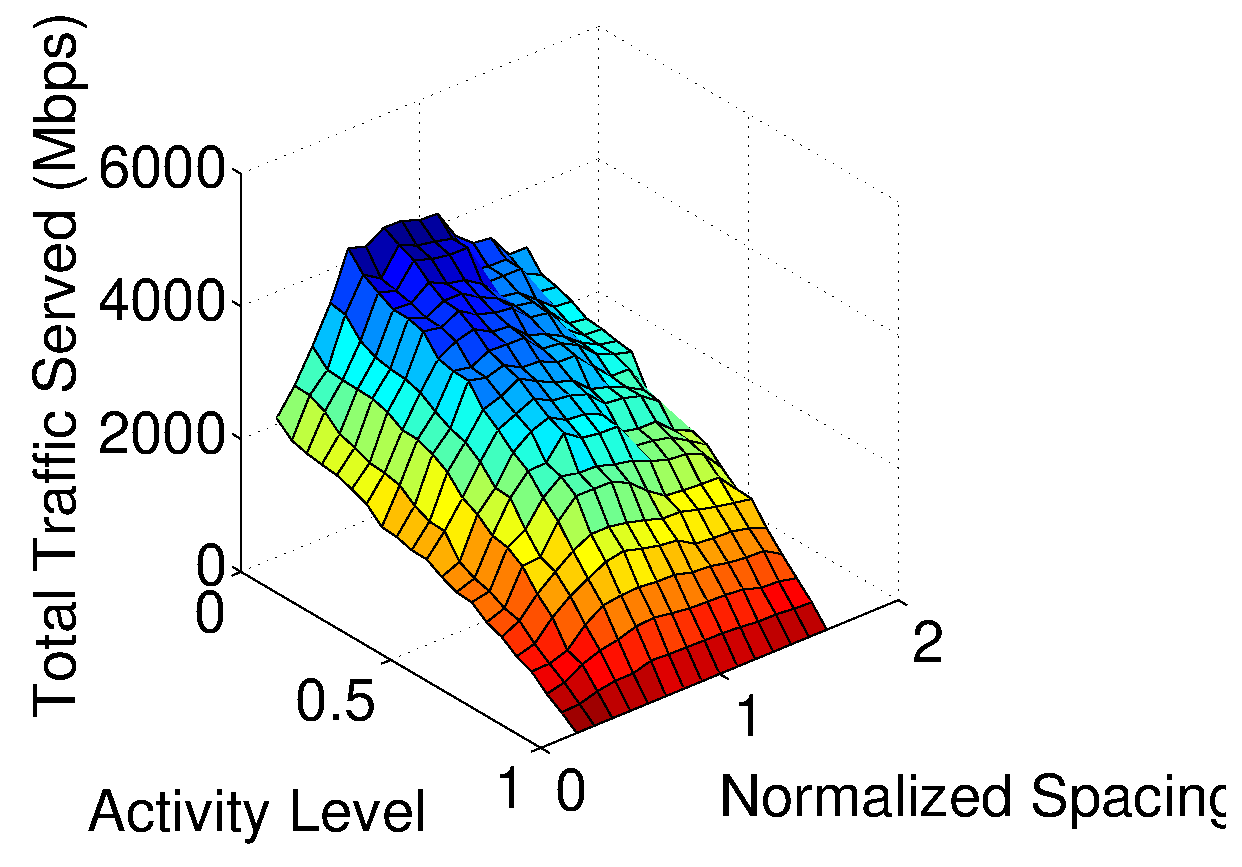
\includegraphics[width=1.6in]{figures/actspac3d}}
\subfigure[Served Traffic Flow with Activity Level \& Spacing ]{
\label{fig:measurespacing}
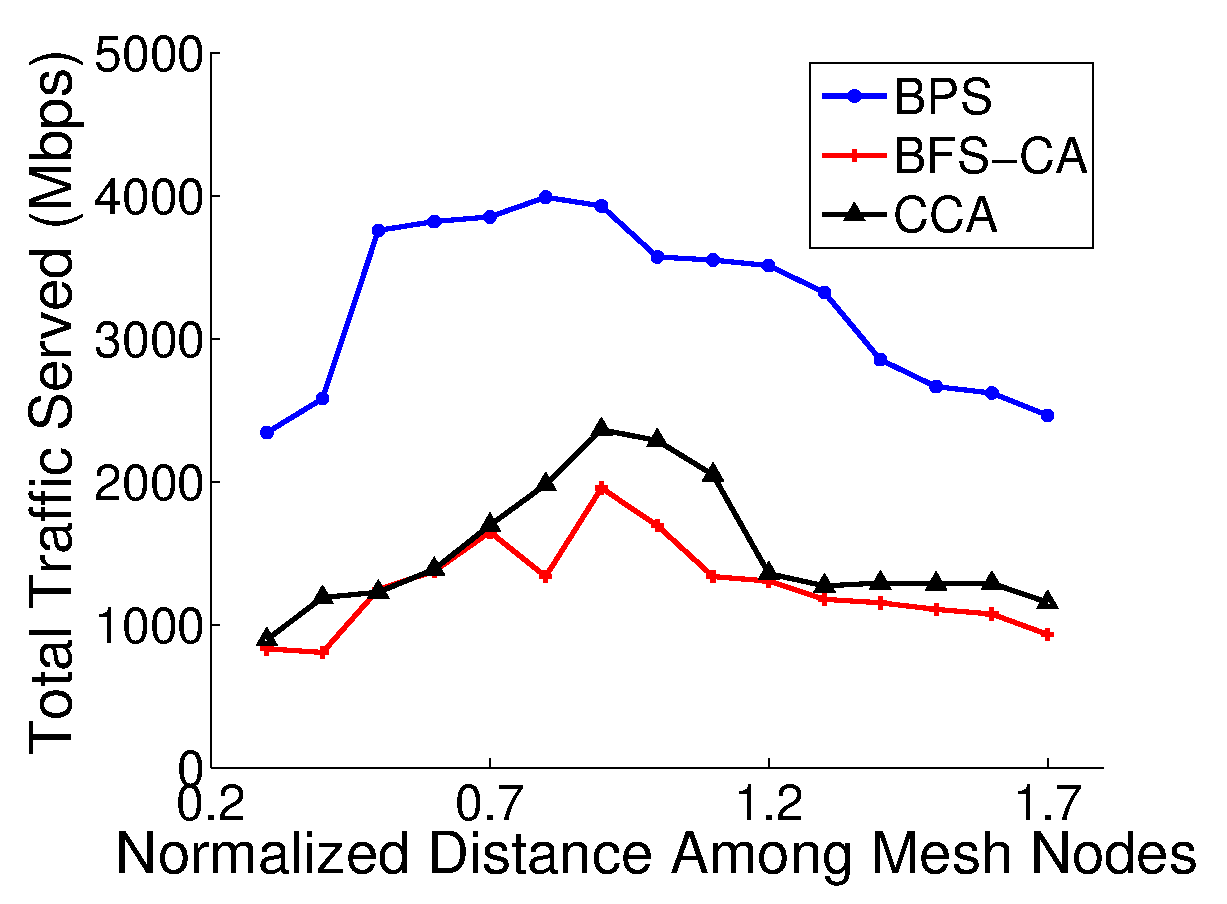
\includegraphics[width=1.6in]{figures/act_spacing}}
\hfill
\caption{Spacing Impacts on the Backhaul Tier}
\label{fig:all3figs}
\vspace{-0.3in}
\end{figure}

In Fig.~\ref{fig:measurespacing}, as the spacing increases, the WhiteMesh network 
has better performance in all methods through spatial reuse, matching the simulation 
analysis shown in Fig.~\ref{fig:actspac}. As the distance increases up to normalized 
distance 1, one of the 5 GHz channels stops working in the network since the distance 
is larger than its communication range. That makes the performance decrease quickly. 

Through this analysis, a mixed WiFi and white space wireless WhiteMesh network 
improves the performance in the following achieve aspects: 
{\it (i)} Heavily utilized networks can get more capacity from spatial reuse and 
flexible path reducing hop count through diverse links. 
{\it (ii)} Rural networks have large mesh spacing to be deployed with a reasonable network performance 
with a fair more reduce of budget.
We are able to find an approaching of optimal WhiteMesh deployment based on this 
analysis.

